% !TEX encoding = UTF-8 Unicode
%Präambel

%Report für große Doukumente. Dieser ist in Kapitel (\chapter{}) aufgeteilt
%\documentclass[12pt, a4paper, ngerman]{report} 

%Article für normale Doumente
\documentclass[12pt, a4paper, ngerman]{article}

%Deutsche Beschreibungen von generiertem Text (table of contents => Inhaltsverzeichnis)
\usepackage[ngerman]{babel}

%Umlaute
\usepackage[utf8]{inputenc}

%Schriftart Helvetica 
\usepackage[scaled]{helvet}

%Seitenränder
\usepackage{geometry}
%top = Abstand nach oben
%left = Abstand nach links
%right = Abstand nach rechts
%bottom= Abstand nach unten
%heapsep= Abstand zwische Kopfzeile und Text
%footskip= Abstand zwischen Text und Fußzeile
\geometry{a4paper, top=25mm, left=30mm, right=25mm, bottom=30mm, headsep=10mm, footskip=12mm}

%Farben nutzen
\usepackage{xcolor}

%Grafiken einbinden
\usepackage{graphicx}

%Zusätzliche Positionsbefehle
\usepackage{float} 

%Die Einrücktiefe bei einem neuen Absatz
\setlength{\parindent}{0pt}

%Fülltext
\usepackage{blindtext}


%Fuer Zitate	
\PassOptionsToPackage{backend=bibtex}{biblatex}
\usepackage[natbib=true,style=numeric]{biblatex}
\usepackage[babel,german=guillemets]{csquotes}
\bibliography{quellen.bib} 

% Aufnahme von \paragraph in das Inhaltsverzeichnis 
\setcounter{tocdepth}{3}  

%Nummerierung vertiefen, \paragraph kommt mit ins Inhaltsverzeichnis
\setcounter{secnumdepth}{4} 

%Feste Tabellen
\usepackage{tabulary}

%caption für nummerierte Tabellenüberschriften
%booktabs für die Steuerung von Linien
\usepackage{caption, booktabs}

%Package fuer Use Cases
\usepackage{useCases}

%Package, um Attribute zu beschreiben
\usepackage{attribute}

%Package, um PDF Dokumente einzubinden
\usepackage{pdfpages} 

%Package um Listings anzuzeigen
\usepackage{listings}

%Rahmen um Listung konfigurieren
\lstset {
     frame=single,               % einfacher Rahmen
     framesep=1pt,               % Abstand des Rahmens
     framerule=0.8pt,            % Linienstaerke des Rahmens
     xleftmargin=1.8pt,          % linker Abstand vom Rand (framesep+framrule)
     xrightmargin=1.8pt,         % rechter Abstand vom Rand (framesep+framrule)
     aboveskip=\medskipamount,   % Abstand vor einer Box
     belowskip=\medskipamount,   % Abstand nach einer Box
}

%Umlaute für Listings konfigurieren
\lstset{literate=%
    {Ö}{{\"O}}1
    {Ä}{{\"A}}1
    {Ü}{{\"U}}1
    {ß}{{\ss}}1
    {ü}{{\"u}}1
    {ä}{{\"a}}1
    {ö}{{\"o}}1
    {~}{{\textasciitilde}}1
}




%Package um die \ref{} zu verlinken. Die Links werden nicht als solche markiert
\usepackage[hidelinks]{hyperref}

%Eigene Kommandos

\newcommand{\todo}[1]{\fcolorbox{red}{yellow}{ \parbox{0.75\linewidth}{#1}}} %To mark tasks can be done, but are not done 
\newcommand{\later}[1]{\fcolorbox{red}{orange}{\parbox{0.75\linewidth}{#1}}} %To mark tasks in the future. Can't be done now (e.g. missing information)
\newcommand{\checked}[1]{\fcolorbox{green}{green}{\parbox{0.75\linewidth}{#1}}} %To mark tasks, containing checked information
\newcommand{\crap}[1]{\fcolorbox{red}{red}{\parbox{0.75\linewidth}{#1}}} %To mark tasks, being absolutely bullshit

\begin{document}

\tableofcontents 
\newpage

\section{Verfügbare Status Marker}

\later{I'm the box marking a task what can not be done at this stadium of the document}

\todo{I'm the box marking a task can be done at this stadium of the document but is not done yet}

\checked{My information are accurate}

\crap{i be the box marks somethimg wrong}
 



\section{Einleitung}
\subsection{Überblick über das Programm}
\todo{kurze Zusammenfassung und Vorstellung}
\subsection{Hintergrund der Datensätze}
\todo{evtl. was über den Hintergrund der Datensätze schreiben}
\subsection{Installationsanleitung und Vorraussetzungen}
Das Programm wurde in C++ realisiert. 
\subsubsection{System}
Getestet wurde die Software auf Mac Books mit Intel CPU.

Das Programm ist UTF-8 kodiert, die eingelesene Datei entspricht auch dieser Kodierung.

Das Programm benötigt in dieser Konfiguration mindestens 160mb Arbeitsspeicher.

\subsubsection{Software}
Auf den Testsystemen war Mac OS 10.9.3 installiert. Zusätzlich war das Softwarepaket Xcode 5.1.1 installiert. 

\textbf{Compiler:}\newline
 g++ 4.2.1  \newline
Apple LLVM version 5.1 (clang-503.0.40) (based on LLVM 3.4svn) \newline
Target: x86\_64-apple-darwin13.2.0 \newline
Thread model: posix


\textbf{IDE:}\newline
Eclipse IDE for C/C++ Developers \newline
Version: Kepler Service Release 2

\subsubsection{Build}
Dem Quellcode liegen makefiles (GNU make) bei.

Bei der Benutzung eigener makefiles ist auf den Schalter \textit{-std=c++11} zu achten. 

Der Quellcode ist ANSI-konform und benutzt keine externen Libraries, wie z.B. Boost.

\subsection{Bedienungsanleitung \label{Bedienungsanleitung}}
\subsubsection{Starten des Programms}
Der Quellcode wird in einem Paket ausgeliefert. Vor der Benutzung der Software muss der Quellcode kompiliert werden. Das Kompilieren erfolgt in den folgenden Schritten:
\begin{enumerate}
	\item Entpacken des Pakets in den Ordner \textit{Routenplaner}\footnote{Bei einem abweichenden Ordnernamen muss dieser im weiteren Verlauf der Installation berücksichtigt werden}. Beim Entpacken dieses Archivs wird ein Verzeichnisbaum unterhalb des Ordners \textit{Routenplaner} erstellt.
	\item Mit dem Kommando \textit|{cd Routenplaner} in den Ordner \textit{Routenplaner} wechseln.
	\item Quellcode mit den Befehl \textit{make} kompilieren.
	\item Starten des Programms mit \textit{./Routenplaner}
\end{enumerate}

Im Ordner \textit{Routenplaner} des Programms muss die Datei \textit{utf8.csv} liegen. Anpassungen von Dateipfad und -Namen können in \ref{hello} erfolgen. Nach dem Entpacken und kompilieren des ausgelieferten Archivs kann das Programm aber ohne Änderungen gestartet werden.

Nach dem Entpacken des Pakets liegt die Datei im Ordner \textit{Routenplaner}. Sollte die Datei beschädigt oder nicht mehr vorhanden sein, muss sie vom Bundesministerium neu angefordert werden. 

\todo{Kann man die einfach runter laden, oder muss die angefordert werden?}

Mögliche Fehler bei der Programminstallation:
\begin{itemize}
	\item Falsches Dateiformat: Bei der Auslieferung des Programms ist die Datei utf8.csv hart eincodiert. Diese Datei ist mit UTF8 kodiert. Der Quelltext des Programms muss im gleichen Format kodiert sein. \todo{Stimmt das denn auch?}
	\item Fehler beim Neu-Kompilieren: Mit dem Befehl \textit{make clean}  werden die vorhandenen Build Dateien gelöscht. Nach dem Löschen kann wieder mit \textit{make } kompiliert werden.
\end{itemize}

\subsubsection{Startknoten wählen}
Nach dem Starten des Programms erscheint die folgende Anzeige:

\begin{lstlisting}

------------Einlesen abgeschlossen-----------


Die Datensaetze werden vorbereitet
Dies kann eine Weile dauern...

0 - um das Programm zu beenden
1 - um den Startknoten zu waehlen
Bitte jetzt waehlen:  
\end{lstlisting}

\todo{Muss das eines Kommentars gewürdigt werden?}

Die Eingabe des Startknotens kann zu Teilen erfolgen und ist case sensitive. So werden beispielsweise mit der Eingabe \textit{sa} alle Knoten gefunden, die \textit{sa} zusammenhängend im Namen haben. Zielt die Suche auf das Finden von \textit{Sa} ab, wird die Suche fehlschlagen. Aufgrund des umfangreichen Datensatzes empfiehlt sich aber eine eine möglichst präzise Angabe. 

Nach der Eingabe von Saarbrücken schlägt das Programm folgende Knoten vor:
\begin{lstlisting}
Knotennummer: 0
Name: Saarbrücken- Rodenhof , "A623"

Knotennummer: 1
Name: Saarbrücken-Johannisbrücke , "L125"
[...]
Knotennummer: 42
Name: Saarbrückenstraße , "B76"
\end{lstlisting} 
Nach dieser Ausgabe kommt die Aufforderung einen Knoten zu wählen:
\begin{lstlisting}
Bitte geben Sie die gewuenschte Nummer des Knoten ein:
\end{lstlisting}

Die Auswahl einer gültigen Knotennummer startet die Distanzberechnung mit diesem Knoten als Startknoten. Diese Berechnung kann, je nach System, eine längere Zeit in Anspruch nehmen. Nachdem die Distanzberechnung abgeschlossen ist ändert sich das Menü.
\begin{lstlisting}
Bitte geben Sie die gewuenschte Nummer des Knoten ein: 29

Der Graph wird berechnet, diese Operation dauert ein wenig.
0 - um das Programm zu beenden
1 - um den Startknoten zu waehlen
2 - um den Zielknoten zu waehlen
\end{lstlisting}

\subsubsection{Zielknoten auswählen}
Das Auswählen des Zielknotens erfolgt analog zu dem Auswählen des Startknotens. Mit der Auswahl des Zielknotens wird die Routenberechnung gestartet. Die Route wird ausgegeben.
\begin{lstlisting}
Bitte geben Sie die gewuenschte Nummer des Knoten ein: 36

Name: Saarbrücken-Wilhelm-Heinrich-Brücke , 
"A620" Entfernung zum Start: 0 Geo Koordninaten: 
49.2337 6.99155

Name: Saarbrücken-Bismarckbrücke , 
"A620" Entfernung zum Start: 1.02447 Geo Koordninaten: 
49.2273 7.00175

Name: Saarbrücken-Sankt Arnual , 
"A620" Entfernung zum Start: 2.45096 Geo Koordninaten: 
49.2197 7.01755

Name: Saarbrücken-Unner , 
"A620" Entfernung zum Start: 3.68308 Geo Koordninaten: 
49.2095 7.02395

Name: Saarbrücken-Unner , 
"B406" Entfernung zum Start: 3.68308 Geo Koordninaten: 
49.2095 7.02395

Name: Saarbrücken-Sankt Arnual , 
"B406" Entfernung zum Start: 4.91519 Geo Koordninaten: 
49.2197 7.01755
\end{lstlisting}

\subsection{Änderungsvorschläge}
Die folgenden Änderungsvorschläge sind ohne großen Aufwand zu implementieren und Verändern die Funktionalität der Software nicht. Die  Änderungen werden erst nach dem neu Kompilieren des Programms und einem Neustart wirksam. 

\subsubsection{Anpassung von Dateipfad und -name}
In der Datei Hello.cpp (\ref{hello}) kann in der Zeile 
\begin{lstlisting}[language=C++]
datei->oeffneDatei("../utf8.csv");
\end{lstlisting}
Der Dateipfad, sowie der Dateiname geändert werden.

\subsubsection{Menüführung}
Die Menüführung ist in der Klasse UserInterface \ref{UserInterface} implementiert. 

\subsubsection{Ausgabe der Lokationen}
Bei der Ausgabe der Lokationen müssen 3 Ausgaben unterschieden werden. Weiterhin erfolgt in den folgenden Methoden keine Ausgabe, es wird lediglich ein String erzeugt, der in der Klasse UserInterface (\ref{UserInterface}) ausgegeben wird.
\paragraph{Ausgabe einer Lokation}
Die Ausgabe einer Lokation kann in den Klassen \ref{class:Gebietslokation}, \ref{class:Linearlokation}, \ref{class:Punktlokation} geändert werden. Bei Änderungen ist die Vererbungshierarchie \ref{fig:klassendiagrammLokations} zu beachten. 

Die Methoden 
\begin{lstlisting}[language=C++]
string Gebietslokation::toString() {...}
string Linearlokation::toString(){...}
string Punktlokation::toString() {...}
\end{lstlisting}
sind dort im Einzelnen anhand der gewünschten Ausgabe anzupassen.

Im Aktuellen Release der Software werden keine Lokationen direkt ausgegeben. 

\paragraph{Ausgabe von Knoten}
Die Ausgabe der Knoten kann in der Klasse Knoten (\ref{class:Knoten}) in der Methode 

\textit{string Knoten"-::toString"-() \{\dots \}} 

angepasst werden.

\paragraph{Ausgabe der berechneten Route}
Die Ausgabe der Knoten einer berechneten Route kann in der Klasse Knoten (\ref{class:Knoten}) in der Methode 

\textit{string Knoten::toStringRoute()\{ \dots \}} 

angepasst werden.


\section{Use Cases}
Im Folgenden wird beschrieben, welche Use Cases das Programm in seiner Release Version bedienen kann. Die Autoren dieser Use Cases sind \glqq Routenplaner \grqq~und \glqq User \grqq. Der Routenplaner ist das Programm, der User ist der Bediener. Use Cases, die rein vom Routenplaner ausgeführt werden, werden automatisiert ausgeführt.

Die Übersicht und Beschreibung der Use Cases sollen das Verständnis fördern, welche Grundfunktionalitäten die Software abseits der Benutzerführung bietet.

\begin{figure}[htbp] 
  \centering
     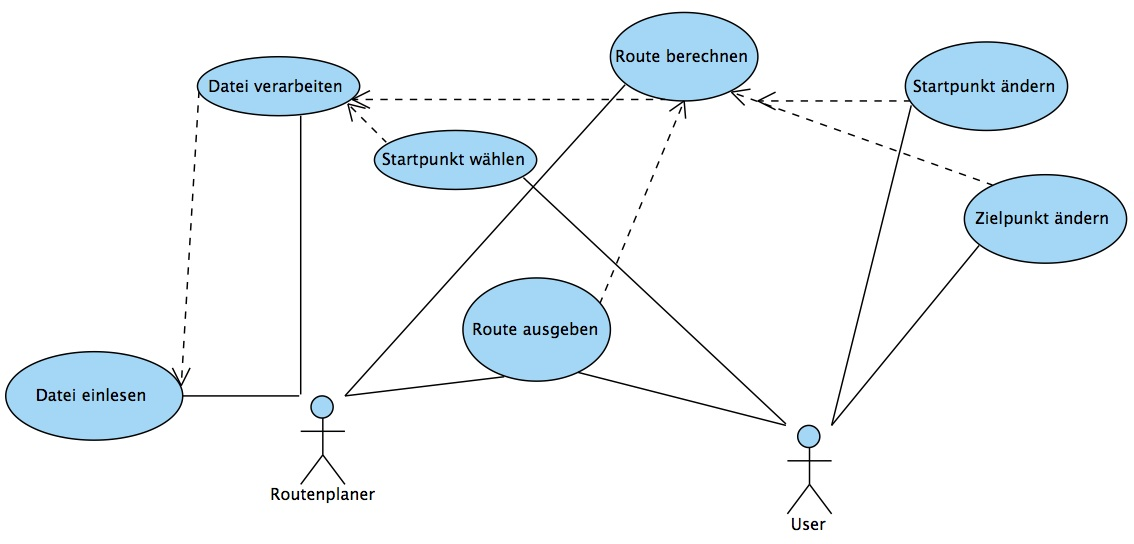
\includegraphics[width=0.9\textwidth]{Grafiken/primaryUseCases.jpg}
  \caption{Übersicht über die Use Cases}
  \label{fig:uebersichtUseCases}
\end{figure}

\subsection{Automatischer Ablauf}
\subsubsection{Datei einlesen \label{uc:DateiEinlesen}}
\begin{usecase}
	\utitle{Datei einlesen}
	\udescription{Nachdem das Programm gestartet wird, wird die csv Datei mit den Streckeninformationen eingelesen.}
	\uactor{Routenplaner}
	\utrigger{Der Start des Programms}
	\uprecondition{Eine gültige Datei mit den Streckeninformationen muss vorliegen, Der richtige Dateiname und -Pfad muss im Programm angegeben sein}
	\upostcondition{Der Inhalt der Datei befindet sich im Arbeitsspeicher}
\end{usecase}

\subsubsection{Datei verarbeiten \label{uc:DateiVerarbeiten}}
\begin{usecase}
	\utitle{Datei verarbeiten}
	\udescription{Aus der bereits eingelesenen Datei werden Objekte erstellt.}
	\uactor{Routenplaner}
	\utrigger{Die Verarbeitung Use Case \ref{uc:DateiEinlesen} ist abgeschlossen}
	\uprecondition{Use Case \ref{uc:DateiEinlesen}}
	\upostcondition{Die primäre Funktionalität des Routenplaners steht dem User zur Verfügung}
\end{usecase}

\subsubsection{Distanzen berechnen \label{uc:RouteBerechnen}}
\begin{usecase}
	\utitle{Distanzen berechnen}
	\udescription{Der Routenplaner berechnet die kürzesten Wege vom Startpunkt zu allen anderen Punkten}
	\uactor{Routenplaner}
	\utrigger{Use Case \ref{uc:StartpunktWaehlen}} 
	\uprecondition{Use Case \ref{uc:DateiVerarbeiten}}
	\upostcondition{Die Distanzen vom Startpunkt zu allen anderen anderen Punkten sind bekannt}
\end{usecase}
\subsection{Abläufe, die vom User angestoßen werden}
\subsubsection{Startpunkt wählen \label{uc:StartpunktWaehlen}}
\begin{usecase}
	\utitle{Startpunkt wählen}
	\udescription{Der User wählt den Startpunkt der Routenberechnung aus}
	\uactor{User}
	\uprecondition{Use case \ref{uc:DateiVerarbeiten}, Der Startpunkt ist ein gültiger Punkt}
	\upostcondition{Die Route wird berechnet}
\end{usecase}

\subsubsection{Startpunkt ändern \label{uc:StartpunktAendern}}
\begin{usecase}
	\utitle{Startpunkt ändern}
	\udescription{Der User ändert den Startpunkt einer bereits berechneten Route}
	\uactor{User}
	\uprecondition{Use case \ref{uc:DateiVerarbeiten}, Der Startpunkt ist ein gültiger Punkt}
	\upostcondition{Die Route wird neu berechnet}
\end{usecase}

\subsubsection{Zielpunkt ändern \label{uc:ZielpunktAendern}}
\begin{usecase}
	\utitle{Zielpunkt ändern}
	\udescription{Der User trägt einen Zielpunkt ein, bzw. ändert einen bestehenden. }
	\uactor{User}
	\uprecondition{\ref{uc:RouteBerechnen}}
	\upostcondition{Der Routenplaner sucht die kürzeste Route und gibt diese aus (Use Case \ref{uc:RouteAusgeben})}
\end{usecase}

\subsubsection{Route ausgeben \label{uc:RouteAusgeben}}
\begin{usecase}
	\utitle{Route ausgeben}
	\udescription{Die kürzeste Route vom Start- zum Zielpunkt wird ausgegeben}
	\uactor{Routenplaner}
	\uprecondition{Use Case \ref{uc:RouteBerechnen},Use Case \ref{uc:ZielpunktAendern}}
\end{usecase}

\section{Verarbeitete Daten \label{attributBeschreibungen}}
Der Routenplaner verarbeitet sämtliche Daten, die im Datensatz vorhanden sind. Da ein Großteil dieser Daten für die Verarbeitung optional ist, werden die notwendigen Daten mit \textit{mandatory} und die optionalen Daten mit \textit{optional} gekennzeichnet. Der Hintergrund, dass die optionalen Daten verarbeitet werden ist, dass optionalen Daten für eine informative Ausgabe benötigt werden können und dem User mehr Komfort bei der Ausgabe bieten können. Die optionalen Daten sind permanent vorhanden und können jederzeit im User Interface abgegriffen und ausgegeben werden.
Die Abbildung \ref{fig:klassendiagrammLokations} zeigt die Hierarchie der Lokationen und deren Attribute.

\begin{figure}[htbp] 
  \centering
     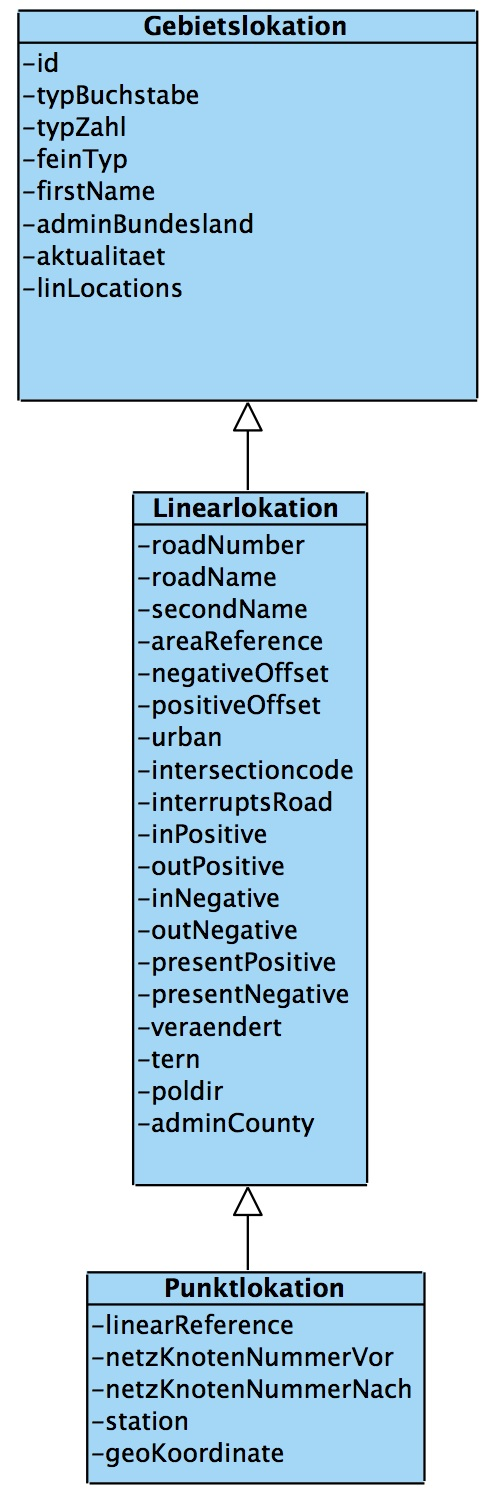
\includegraphics[width=0.3\textwidth]{Grafiken/klassenDiagrammLokations.jpg}
  \caption{Hierarchie der Lokationsklassen}
  \label{fig:klassendiagrammLokations}
\end{figure}

Der originale Datensatz wurde in drei Klassen nachgebildet. Diese entsprechen auch den verschiedenen Location, die in der original Dokumentation des Bundes beschrieben sind.
\subsection{Gebietslokation \label{AreaLocation}}
Eine Area Location, oder Gebietslokation, ist ein grobes Gebiet. Gebiete können beispielsweise Kontinente, Länder, Bundesländer oder Ballungsgebiete sein. Sie stellt den Grundtyp der anderen Lokalionen dar.

\begin{attribut}{Id}
	\drequired{ja}
	\dtype{unsigned int}
	\dmapping{LOCATIONCODE}{Id}
	\dbeschreibung{Eine Id ist einer Lokation eindeutig zugeordnet. Sie wird mit aus dem Datensatz ausgelesen und fest mit dem Objekt verbunden.}
\end{attribut}

\begin{attribut}{typBuchstabe}
	\drequired{nein}
	\dtype{char}
	\dmapping{TYPE}{typBuchstabe + typZahl}
	\dbeschreibung{Dieses Attribut gibt an, um welchen Typ von Lokation es sich handelt. Der ursprüngliche Datentyp besteht aus der Kombination \textless Art der Lokation\textgreater \textless Beschreibung\textgreater. Die Art der Lokation ist ein Buchstabe, der in diesem Attribut gespeichert wird.}
	\dbelegung{A - Gebietslokation, L - Linearlokation, P - Punktlokation }
\end{attribut}

\begin{attribut}{typZahl}
	\drequired{nein}
	\dtype{int}
	\dmapping{TYPE}{typBuchstabe + typZahl}
	\dbeschreibung{Dieses Attribut beschreibt die Lokation genauer. Der ursprüngliche Datentyp besteht aus der Kombination \textless Art der Lokation\textgreater \textless Beschreibung\textgreater. Die genauere Beschreibung der Lokation ist eine Zahl.}
	\dbelegung{Die Zuordnung der Zahlen kann dem Dokument \ref{bundFeinDoku} entnommen werden. Zu beachten ist hierbei\, dass für verschiedene Lokationen andere Zahlenschlüssel gelten.}
\end{attribut}
Die Beschreibung von Lokationen kann weiter herunter gebrochen werden. Die Beschreibung, welche Zahlenwerte hierfür zur Verfügung stehen findet im angehängten Dokument unter \ref{bundFeinDoku}.

\begin{attribut}{feinTyp}
	\drequired{nein}
	\dtype{int}
	\dmapping{SUBTYPE}{feinTyp}
	\dbeschreibung{Der feinTyp beschreibt den Typ einer Lokation genauer. Der Typ A5 beispielsweise steht für ein Gewässer. Wird das Gewässer durch den Feintyp 2 genauer spezifiziert, wird das allgemeine Gewässer zu einem Binnensee.}
	\dbelegung{Siehe \ref{bundFeinDoku}. Dort in der Spalte \glqq Untertyp\grqq~beschrieben}	
\end{attribut}

\begin{attribut}{firstName}
	\drequired{ja}
	\dtype{string}
	\dmapping{FIRST\_NAME}{firstName}
	\dbeschreibung{Der firstName ist der Name der Lokation. Dies kann beispielsweise \glqq Deutschland\grqq~oder \glqq Wallerfangen\grqq~sein. }
\end{attribut}

\begin{attribut}{aktualitaet}
	\drequired{nö}
	\dtype{Aktualitaet*}
	\dmapping{ACTUALITY}{aktualitaet}
	\dbeschreibung{Die aktualitaet beschreibt vermutlich das Erstelldatum der Lokation. In \ref{bundAttributListe} ist dieses Datenfeld nicht dokumentiert. Anhand den aufgetretenen Werten wurde ermittelt, dass es sich dabei um ein Datum handeln muss. Der Wertebereich liegt grob zwischen 2008 und 2013. Die Vermutung, dass dieses Datenfeld das Erstelldatum oder Einpfegedatum der Lokation ist, stützt sich auf den Namen und den Wertebereich. Die Aktualitaet Klasse  \ref{class:Aktualitaet} im Programm stützt sich auf ein \glqq tm *zeit\grqq~struct, ist aber komfortabler zu nutzen.}
\end{attribut}

\begin{attribut}{linLocations}
	\drequired{nope}
	\dtype{vector\textless Linearlokation*\textgreater}
	\dbeschreibung{Jede Gebietslokation hat die Linearlokationen \ref{linearLokation}, die diese Gebietslokation als übergeordnet angegeben hat in einem Vector gespeichert.}
\end{attribut}

\subsection{Linearlokation \label{linearLokation}}

\begin{attribut}{roadNumber}
	\drequired{nein}
	\dtype{string}
	\dmapping{ROADNUMBER}{roadNumber}
	\dbeschreibung{Die roadNumber gibt die Nummer der Straße nach der Einteilung von Bund und Ländern an. Sie ist mit einem führenden Buchstaben und einer Nummer angegeben. Ein Beispiel für eine roadNumber ist \glqq A620\grqq. Neben den bekannten Bezeichnungen ist auch die Bezeichnung \glqq GDD\grqq aufgetreten. Diese Bezeichnung stammt von einem privaten Anbieter. Näheres dazu gibt es im Kapitel \ref{bundGDD}}
\end{attribut}

\begin{attribut}{roadName}
	\drequired{nein}
	\dtype{string}
	\dmapping{ROADNAME}{roadName}
	\dbeschreibung{Der roadName ist der Name einer Straße. Dieses Attribut darf nicht mit \ref{dt:roadNumber} verwechselt werden. Ein Beispiel für einen roadName ist \glqq Metzer Straße\glqq. Diese Straße hat die roadNumber \glqq B406\grqq.}
\end{attribut}

\begin{attribut}{secondName}
	\drequired{nein}
	\dtype{string}
	\dmapping{SECOND\_NAME}{secondName}
	\dbeschreibung{Der secondName ist ein zusätzlicher Name einer Lokation. Ein Beispiel hierfür ist die Straße \glqq GDD12\grqq, \glqq Budapester Straße\grqq, \glqq Georgplatz\grqq, wobei die dritte Angabe der socondName ist.}
\end{attribut}

\begin{attribut}{areaReference}
	\drequired{nein}
	\dtype{Gebietslokation*}
	\dmapping{AREA\_REFERENCE}{areaReference}
	\dbeschreibung{Jede Linear Location hat eine übergeordnete Area Location \ref{AreaLocation}. Dieses Attribut ist ein Pointer auf diese übergeordnete Area Lokation.}
\end{attribut}

\begin{attribut}{negativeOffset}
	\drequired{ja}
	\dtype{Linearlokation*}
	\dmapping{NEGATIVE\_OFFSET}{negativeOffset}
	\dbeschreibung{Der negativeOffset ist grundsätzlich eine vorangehende oder nachfolgende Linear Location. Laut der Beschreibung des Bundes eine Vorgängerlokation bezogen auf die Erfassungsrichtung. Das Attribut ist als Pointer angelegt und erlaubt eine Bewegung durch die Lokationen. Für die Distanzberechnung wurde angenommen, dass es zwischen den Offset eine direkte Verbindung gibt.}
\end{attribut}

\begin{attribut}{positiveOffset}
	\drequired{ja}
	\dtype{Linearlokation*}
	\dmapping{POSITIVE\_OFFSET}{positiveOffset}
	\dbeschreibung{Siehe Attribut \ref{dt:negativeOffset}. Im Gegensatz zum negativeOffset wird der positiveOffset als eine Nachfolgelokation bezogen auf die Erfassungsrichtung beschrieben.}
\end{attribut}

\begin{attribut}{urban}
	\drequired{nein}
	\dtype{bool}
	\dmapping{URBAN}{urban}
	\dbeschreibung{Flag, ob Verkehr städtischen Charakters vorliegt.}
	\dbelegung{0 = nein = false, 1 = ja = true }
\end{attribut} 	
	

\begin{attribut}{intersectioncode}
	\drequired{ja}
	\dtype{Linearlokation*}
	\dmapping{INTERSECTIONSCODE}{intersectioncode}
	\dbeschreibung{Der intersectioncode ist ein Pointer auf eine andere Linear Location, die die aktuelle Linear Location kreuzt. Bei der Distanzberechnung wird sie als potenzieller Nachfolger angenommen. Aus den Datensätzen ist nicht ersichtlich, ob der Intersectioncode tatsächlich eine Verbindung zu der aktuellen Linear Location hat. Näheres dazu steht im Kapitel \ref{Probleme}}
\end{attribut}

\begin{attribut}{interruptsRoad}
	\drequired{nein}
	\dtype{Linearlokation*}
	\dmapping{INTERRUPTS\_ROAD}{interruptsRoad}
	\dbeschreibung{\todo{Hast du noch im Kopf, was das Ding konnte?}}
\end{attribut}

\begin{attribut}{inPositive}
	\drequired{nein}
	\dtype{bool}
	\dmapping{IN\_POSITIVE}{inPositive}
	\dbeschreibung{inPositive beschreibt, ob die Lotion in Erfassungsrichtung zugänglich ist. }
	\dbelegung{0 = nein = false, 1 = ja = true}
\end{attribut}

\begin{attribut}{outPositive}
	\drequired{nein}
	\dtype{bool}
	\dmapping{OUT\_POSITIVE}{outPositive}
	\dbeschreibung{outPositive beschreibt, ob die Lotion in Erfassungsrichtung verlassen werden kann. }
	\dbelegung{0 = nein = false, 1 = ja = true}
\end{attribut}


\begin{attribut}{inNegative}
	\drequired{nein}
	\dtype{bool}
	\dmapping{IN\_NEGATIVE}{inNegative}
	\dbeschreibung{inNegative beschreibt, ob die Lotion entgegen der Erfassungsrichtung zugänglich ist. }
	\dbelegung{0 = nein = false, 1 = ja = true}
\end{attribut}

\begin{attribut}{outNegative}
	\drequired{nein}
	\dtype{bool}
	\dmapping{OUT\_NEGATIVE}{outNegative}
	\dbeschreibung{outPositive beschreibt, ob die Lotion entgegen der Erfassungsrichtung verlassen werden kann.}
	\dbelegung{0 = nein = false, 1 = ja = true}
\end{attribut}


\begin{attribut}{presentPositive}
	\drequired{nein}
	\dtype{bool}
	\dmapping{PRESENT\_POSITIVE}{presentPositive}
	\dbeschreibung{outPositive beschreibt, ob die Lotion in Erfassungsrichtung vorhanden ist.}
	\dbelegung{0 = nein = false, 1 = ja = true}
\end{attribut}


\begin{attribut}{presentNegative}
	\drequired{nein}
	\dtype{bool}
	\dmapping{PRESENT\_NEGATIVE}{inNegative}
	\dbeschreibung{presentNegative beschreibt, ob die Lotion entgegen der Erfassungsrichtung vorhanden ist}
	\dbelegung{0 = nein = false, 1 = ja = true}
\end{attribut}

\begin{attribut}{veraendert}
	\drequired{nein}
	\dtype{int}
	\dmapping{VER\"ANDERT}{veraendert}
	\dbeschreibung{Flag, ob Datensatz bei Aktualisierungslauf gegenüber der Vorgängerversion verändert wurde (nur vor Release erkennbar). Im vorliegenden Datensatz war veraendert in jeder Location == 0}
	\dbelegung{0 - nein, 1 - ja, 3 - löschen}
\end{attribut}


\begin{attribut}{tern}
	\drequired{nein}
	\dtype{bool}
	\dmapping{TERN}{tern}
	\dbeschreibung{Angabe, ob Lokation zum TERN-Netz gehört.}
	\dbelegung{0 = nein = false, 1 = ja = true}
\end{attribut}
	
\begin{attribut}{poldir}
	\drequired{nein}
	\dtype{string}
	\dmapping{POLDIR}{poldir}
	\dbeschreibung{Hinweis auf die nächste zuständige Polizeibehörde.}	
\end{attribut}
	

\begin{attribut}{adminBundesLand}
	\drequired{nein}
	\dtype{string}
	\dmapping{ADMIN\_County}{adminBundesLand}
	\dbeschreibung{Der adminBundesLand gibt an, welches Bundesland für die Bearbeitung dieser Lokation zuständig ist. }
	\dbelegung{BW - Baden-Württemberg, BY - Bayern, BE - Berlin, BB - Brandenburg, HB - Bremen, HH - Hamburg, HE - Hessen, MV - Mecklenburg-Vorpommern, NI - Niedersachsen, NW - Nordrhein-Westfalen, RP - Rheinland-Pfalz, SL - Saarland, SN - Sachsen, ST - Sachsen-Anhalt, SH - Schleswig-Holstein, TH - Thüringen}
\end{attribut}
	
\subsection{Punktlokation \label{Punklokation}}
\begin{attribut}{linearReference}
	\drequired{nein}
	\dtype{Linearlokation*}
	\dmapping{LINEAR\_REFERENCE}{linearReference}
	\dbeschreibung{Eine Punktlokation hat eine übergeordnete Linearlokation \ref{LinearLokation}. Dieses Attribut ist ein Pointer auf diese Linearlokation. }
\end{attribut}

\begin{attribut}{netzKontenNummerVor}
	\drequired{nein}
	\dtype{unsigned int}
	\dmapping{NETZKNOTEN1\_NR}{netzKnotenNummerVor}
	\dbeschreibung{Netzknotennummer der Lokation oder Netzknotennummer des vor der Lokation liegenden Netzknoten. Im Datensatz sind diese Datenfelder zwar gesetzt, aber einen Zusammenhang oder einen Sinn konnten wir nicht feststellen.}
\end{attribut}

\begin{attribut}{netzKontenNummerNach}
	\drequired{nein}
	\dtype{unsigned int}
	\dmapping{NETZKNOTEN2\_NR}{netzKnotenNummerNach}
	\dbeschreibung{Netzknotennummer des nach der Lokation liegenden Netzknoten. Im Datensatz sind diese Datenfelder zwar gesetzt, aber einen Zusammenhang oder einen Sinn konnten wir nicht feststellen.}
\end{attribut}

\begin{attribut}{station}
	\drequired{nein}
	\dtype{int}
	\dmapping{STATION}{station}
	\dbeschreibung{Entfernung der Lokation vor dem netzKontenNummerVor in Richtung netzKontenNummerNach. Die Angabe ist in Metern. Da sich uns nicht der Sinn der Netzknoten erschlossen hat, ergibt dieses Attribut auch keinen Sinn.}
\end{attribut}

\begin{attribut}{geoKoordinate}
	\drequired{ja}
	\dtype{GeoKoordinate*}
	\dmapping{X-KOORDINATE + Y-KOORDINATE}{geoKoordinate}
	\dbeschreibung{Ein GeoKoordinate Objekt enthält eine Position mit WGS84 Koordinaten. Es beinhaltet Methoden um Distanzen zwischen gegebenen Positionen oder anderen GeoKoordinate Objekten zu berechnen. Dieses Attribut ist ein Pointer auf das GeoKoordinate Objekt der aktuellen Punktlokation.}
\end{attribut}	


\section{Programmablauf}
In diesem Kapitel wird beschrieben, wie die einzelnen Ablaufschritte des Programms voneinander abhängen. Die Betrachtung der Abläufe ist eine Ergänzung zu den Use Cases und deutlich differenzierter.

\subsection{Datei Verarbeitung}

\begin{figure}[H] 
  \centering
     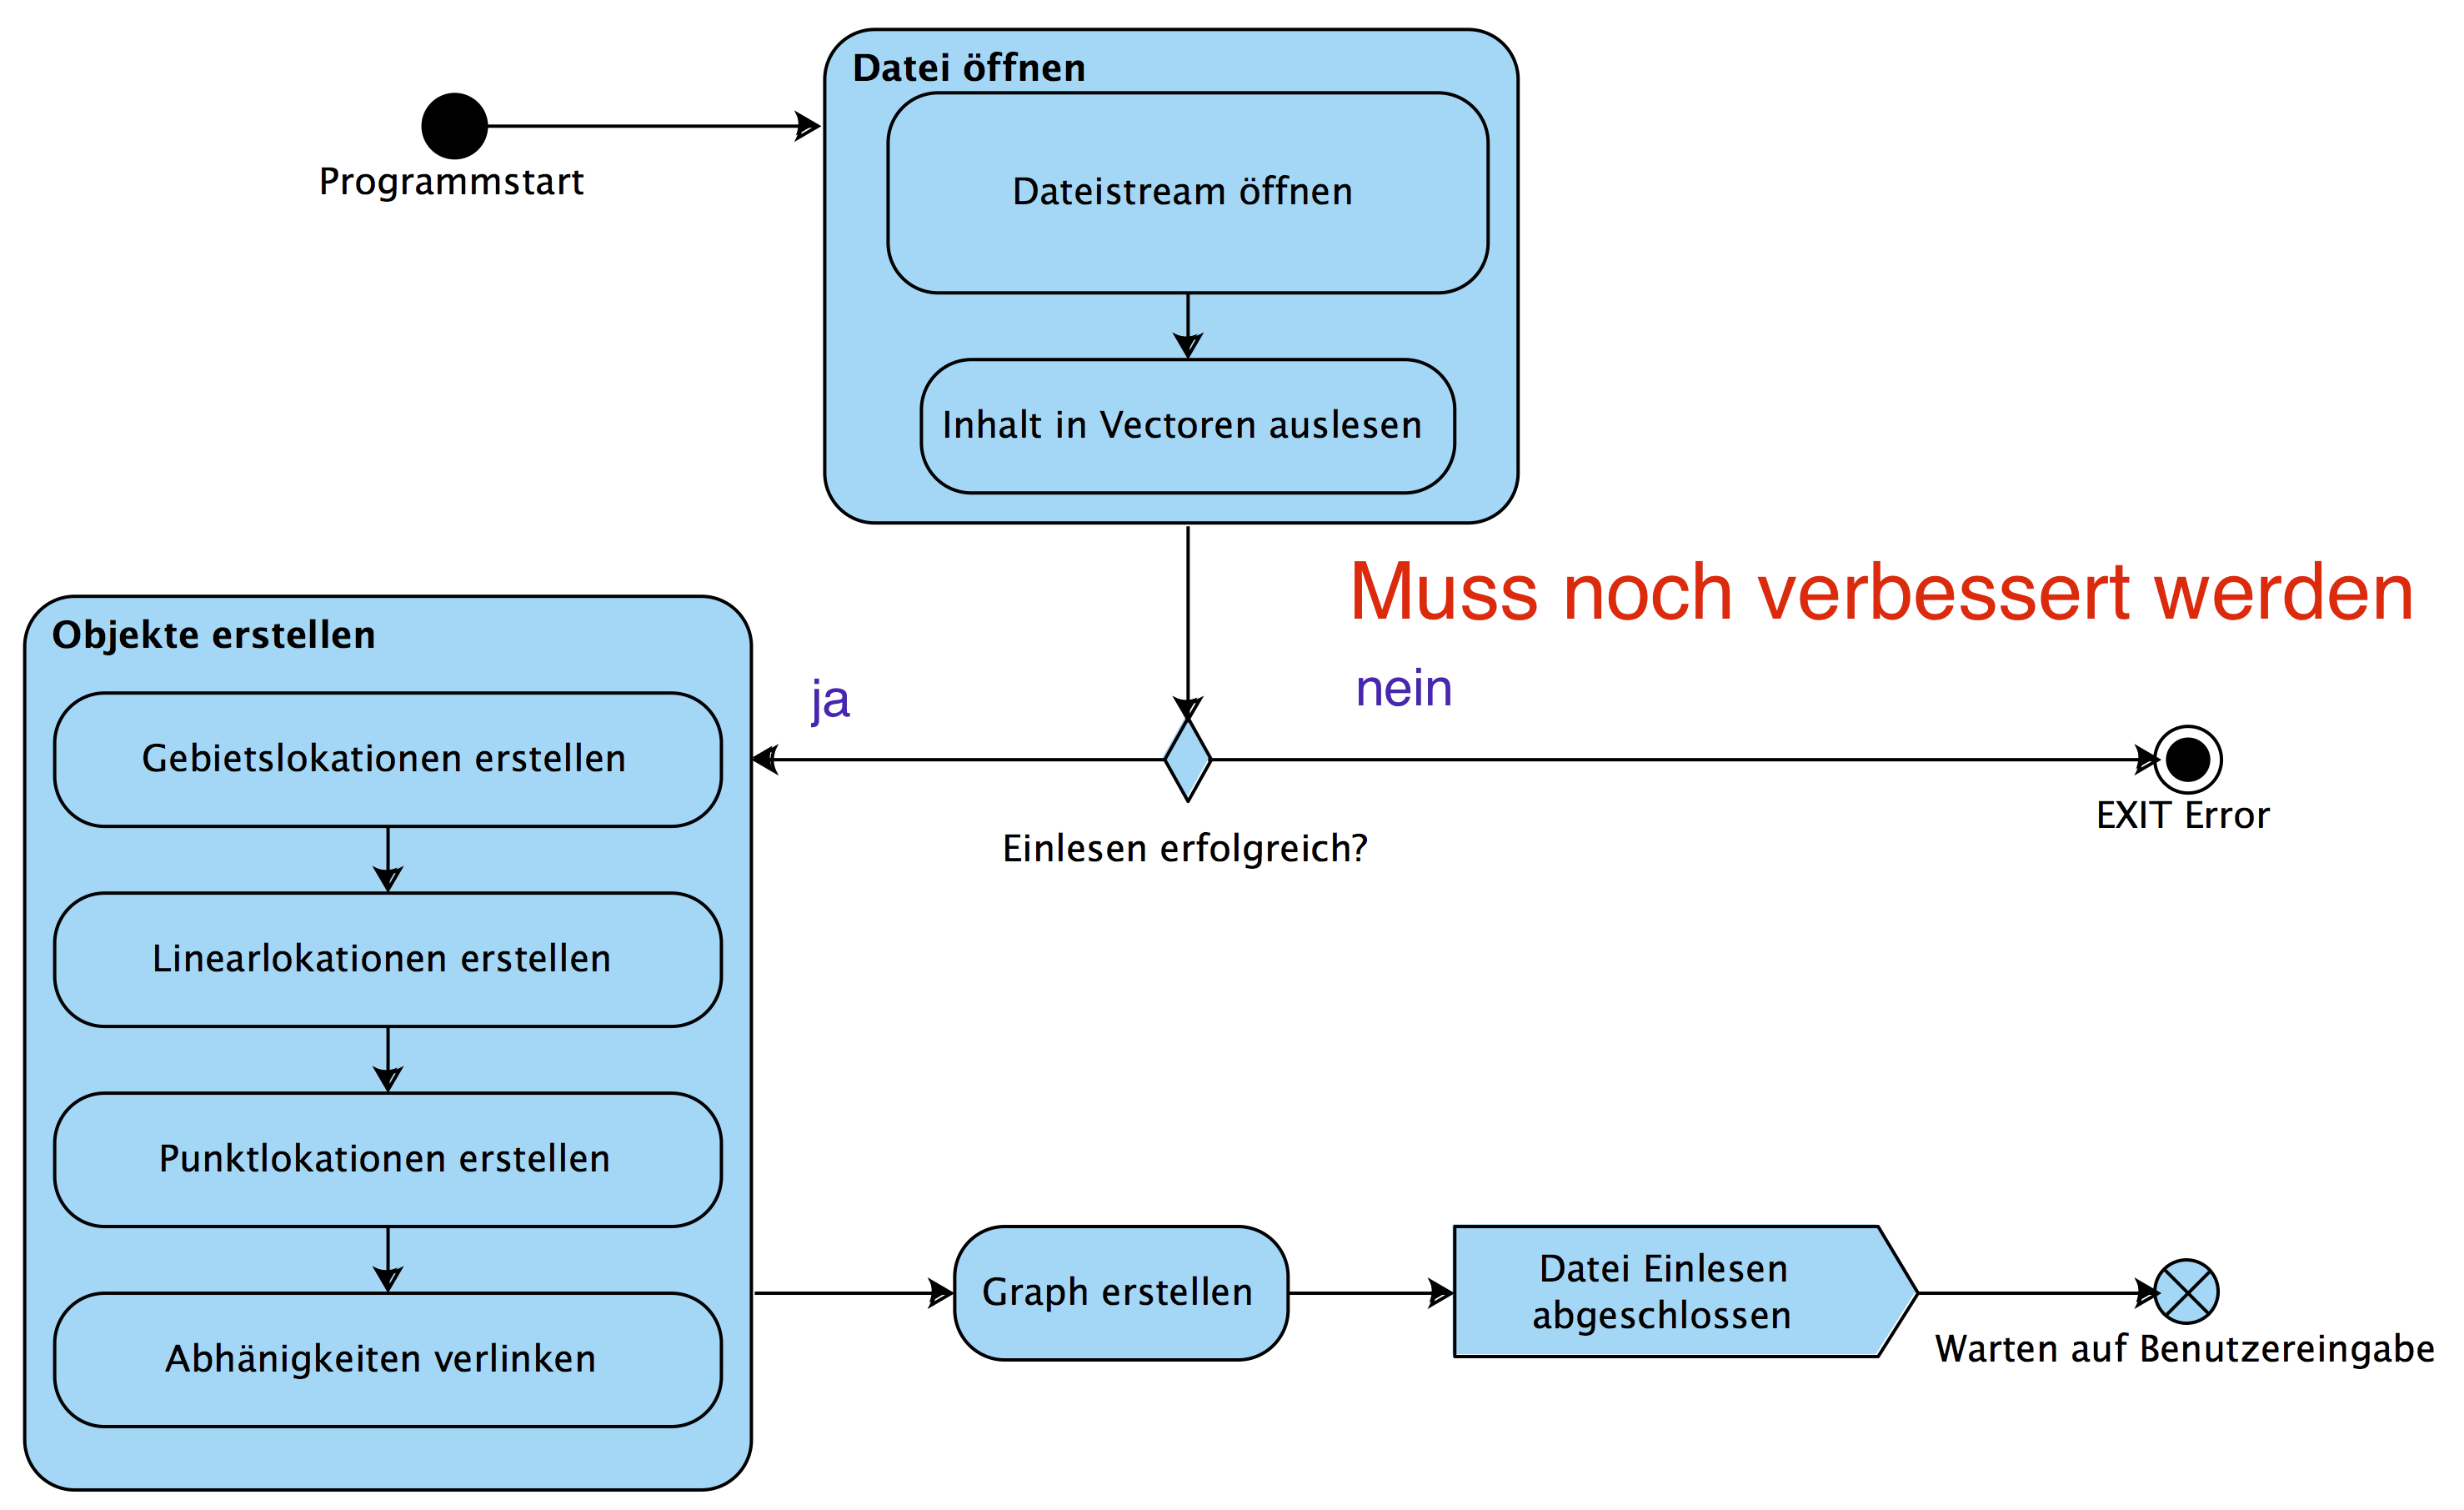
\includegraphics[width=1.0\textwidth]{Grafiken/aktivitaetsDiagrammDateiEinlesen.jpg}
  \caption{Aktivitätsdiagramm des Dateieinlesens}
  \label{fig:uebersichtDateiEinlesen}
\end{figure}

\subsubsection{Datei öffnen \label{dateiOeffnen}}
Die Aktivität Datei öffnen besteht aus zwei Aktionen. Der erste Schritt ist, die Datei in einen Filestream zu ziehen. Nachdem dieser Filestream geöffnet wurde, wird die Datei zeilenweise in Strings eingelesen. Diese Strings werden anhand des Zeichens \glqq ;\grqq~weiter zerlegt. Das Ergebnis ist eine Matrix, die in einem \textit{vector\textless vector\textless string\textgreater \textgreater} gespeichert ist.

Datei Pfad und -Name sind fest in das Programm einkodiert und können vom Enduser nicht geändert werden. Wenn das Einlesen der Datei fehlschlägt, wird das Programm mit einer Fehlermeldung beendet.

Die Klassen die Das Einlesen der Datei übernimmt heißt FileOpener (\ref{class:FileOpener})
\subsubsection{Objekte erstellen \label{objekteErstellen}}
Die Erstellung und Verwaltung der Lokationsobjekte findet in der Klasse \textit{LokationsVerwaltung} statt. 

Das Erstellen der Lokationsobjekte läuft in vier Schritten ab. Der Hintergrund ist, dass die Objekte untereinander Abhängigkeiten haben, die für einen schnelleren Zugriff als Pointer gespeichert sind. Eine Gebietslokation  \ref{AreaLocation} hat beispielsweise Pointer auf ihre untergeordneten Linearlokationen \ref{linearLokation} gespeichert, während die Linearlokationen Pointer auf ihre übergeordneten Gebietslokationen gespeichert haben.

Um einen sicheren Zugriff auf die Elemente einer Spalte zu garantieren, sind in der Datei \textit{AttributDefines.h} die entsprechenden Stellen der Elemente als Defines gespeichert.

Die Objekte werden dynamisch allokiert und Pointer auf sie werden in einer Map gespeichert.  

Diese Objekte bieten den Grund Datenbestand. Auf diesen Datenbestand werden können Suchen ausgeführt werden und aus diesem Datenbestand werden die Informationen für die Ausgaben entnommen. Außerdem basiert der Graph auf diesem Datenbestand.

\paragraph{Gebietslokationen erstellen \label{par:gebietsLokationenErstellen}}
Im ersten Schritt des Durchlaufs werden die Gebietslokationen eingelesen. Dazu wird der Vector zeilenweise durchlaufen. Wenn der Typ einer Zeile mit einem \glqq A\grqq  beginnt wird ein Gebietslokation Objekt erstellt.

\paragraph{Linearlokationen erstellen}
Nach der Erstellung der Gebietslokationen werden die Linearlokationen erstellt. Die Pointer dieser Linearlokationen werden direkt in die Listen der übergeordneten Gebietslokationen eingepflegt. Parallel dazu werden die Pointer der übergeordneten Gebietslokationen \ref{dt:areaReference} in die Linearlokationen eingetragen. Der Prozess des Einlesens läuft analog zu \ref{par:gebietsLokationenErstellen}. Die Zeilen müssen aber mit \glqq L \grqq beginnen. 

\paragraph{Punktlokationen erstellen}
Nach den Linearlokationen werden die Punktlokationen erstellt. Die Pointer der erstellten Punktlokationen werden direkt in die Listen der übergeordneten Linearlokationen eingetragen. Beim Erstellen der Punktloationen werden die Pointer auf übergeordneten Linearlokationen \ref{dt:linearReference} direkt eingetragen. Der Prozess des Einlesens läuft analog zu \ref{par:gebietsLokationenErstellen}. Die Zeilen müssen aber mit \glqq P \grqq beginnen. 


\paragraph{Abhängigkeiten verlinken} 
Der vierte Schritt ist das Verlinken der Abhängigkeiten. In diesem Schritt werden die Pointer der Offset (\ref{dt:negativeOffset} und \ref{dt:positiveOffset}), sowie die Pointer von InterruptsRoad \ref{dt:interruptsRoad} und IntersectionCode \ref{dt:intersectioncode} in die jeweiligen Objekte eingetragen. Dazu wird wieder Zeile für Zeile ausgelesen. Aus der Zeile werden die Id an den entsprechenden Stellen ausgelesen. Anhand dieser Id werden die Pointer der entsprechenden Objekte gesucht und in die Attribute der jeweiligen Lokationen eingetragen.

\subsubsection{Graph erstellen}
Der Graph ist ähnlich aufgebaut, wie der Grunddatenbestand. Er besteht aus einer Liste mit Knoten. Zusätzlich bietet die Klasse \textit{Graph}  Methoden um den Graph aufzubauen und zu pflegen. Das Erstellen des Graphen läuft schrittweise ab.

\paragraph{Erstellen der Knoten \label{knotenErstellen}}
Ein Knoten ist ein eigenes Objekt. Er enthält einen Pointer auf die Punktlokation, die der Knoten darstellt. Weiterhin hat ein Knoten eine Liste mit Pointern von weiteren Knoten, die vom Streckenverlauf her seine Nachfolger sind, einen Pointer auf seinen Vorgänger, eine Distanz zum Startknoten und ein Flag, ob er bereits besucht wurde. Der Ausdruck Nachfolger bezieht sich auf die Knoten, die er direkt erreichen kann, bzw. die Punktlokationen, die von seiner Punktloaktion aus erreicht werden können. Die Richtung, die in den originalen Datensätzen beschrieben wird spielt hierbei keine Rolle.

Bei der Erstellung der Knoten wird der Grunddatenbestand durchlaufen. Wenn eine Lokation eine Punktlokation ist, wird mit ihr ein Knoten erstellt. 

\paragraph{Verlinken der Knoten} 
Beim Verlinken der Knoten wird die Liste mit den gerade erstellten Knoten durchlaufen. Bei jedem Knoten wird geprüft, welche Punktlokationen von der ihm zu Grunde liegenden Punktloaktion erreicht werden können. Die auf diesen Punklokation basierenden Knoten werden gesucht und als Nachfolger eingetragen.

\subsubsection{Warten auf Benutzereingabe}
Wenn das Verlinken der Knoten abgeschlossen ist, ist auch das Einlesen der Datei beendet. Das Programm wartet ab dieser Stelle auf eine Benutzereingabe.

\subsection{Routenberechnung}

\begin{figure}[H] 
  \centering
     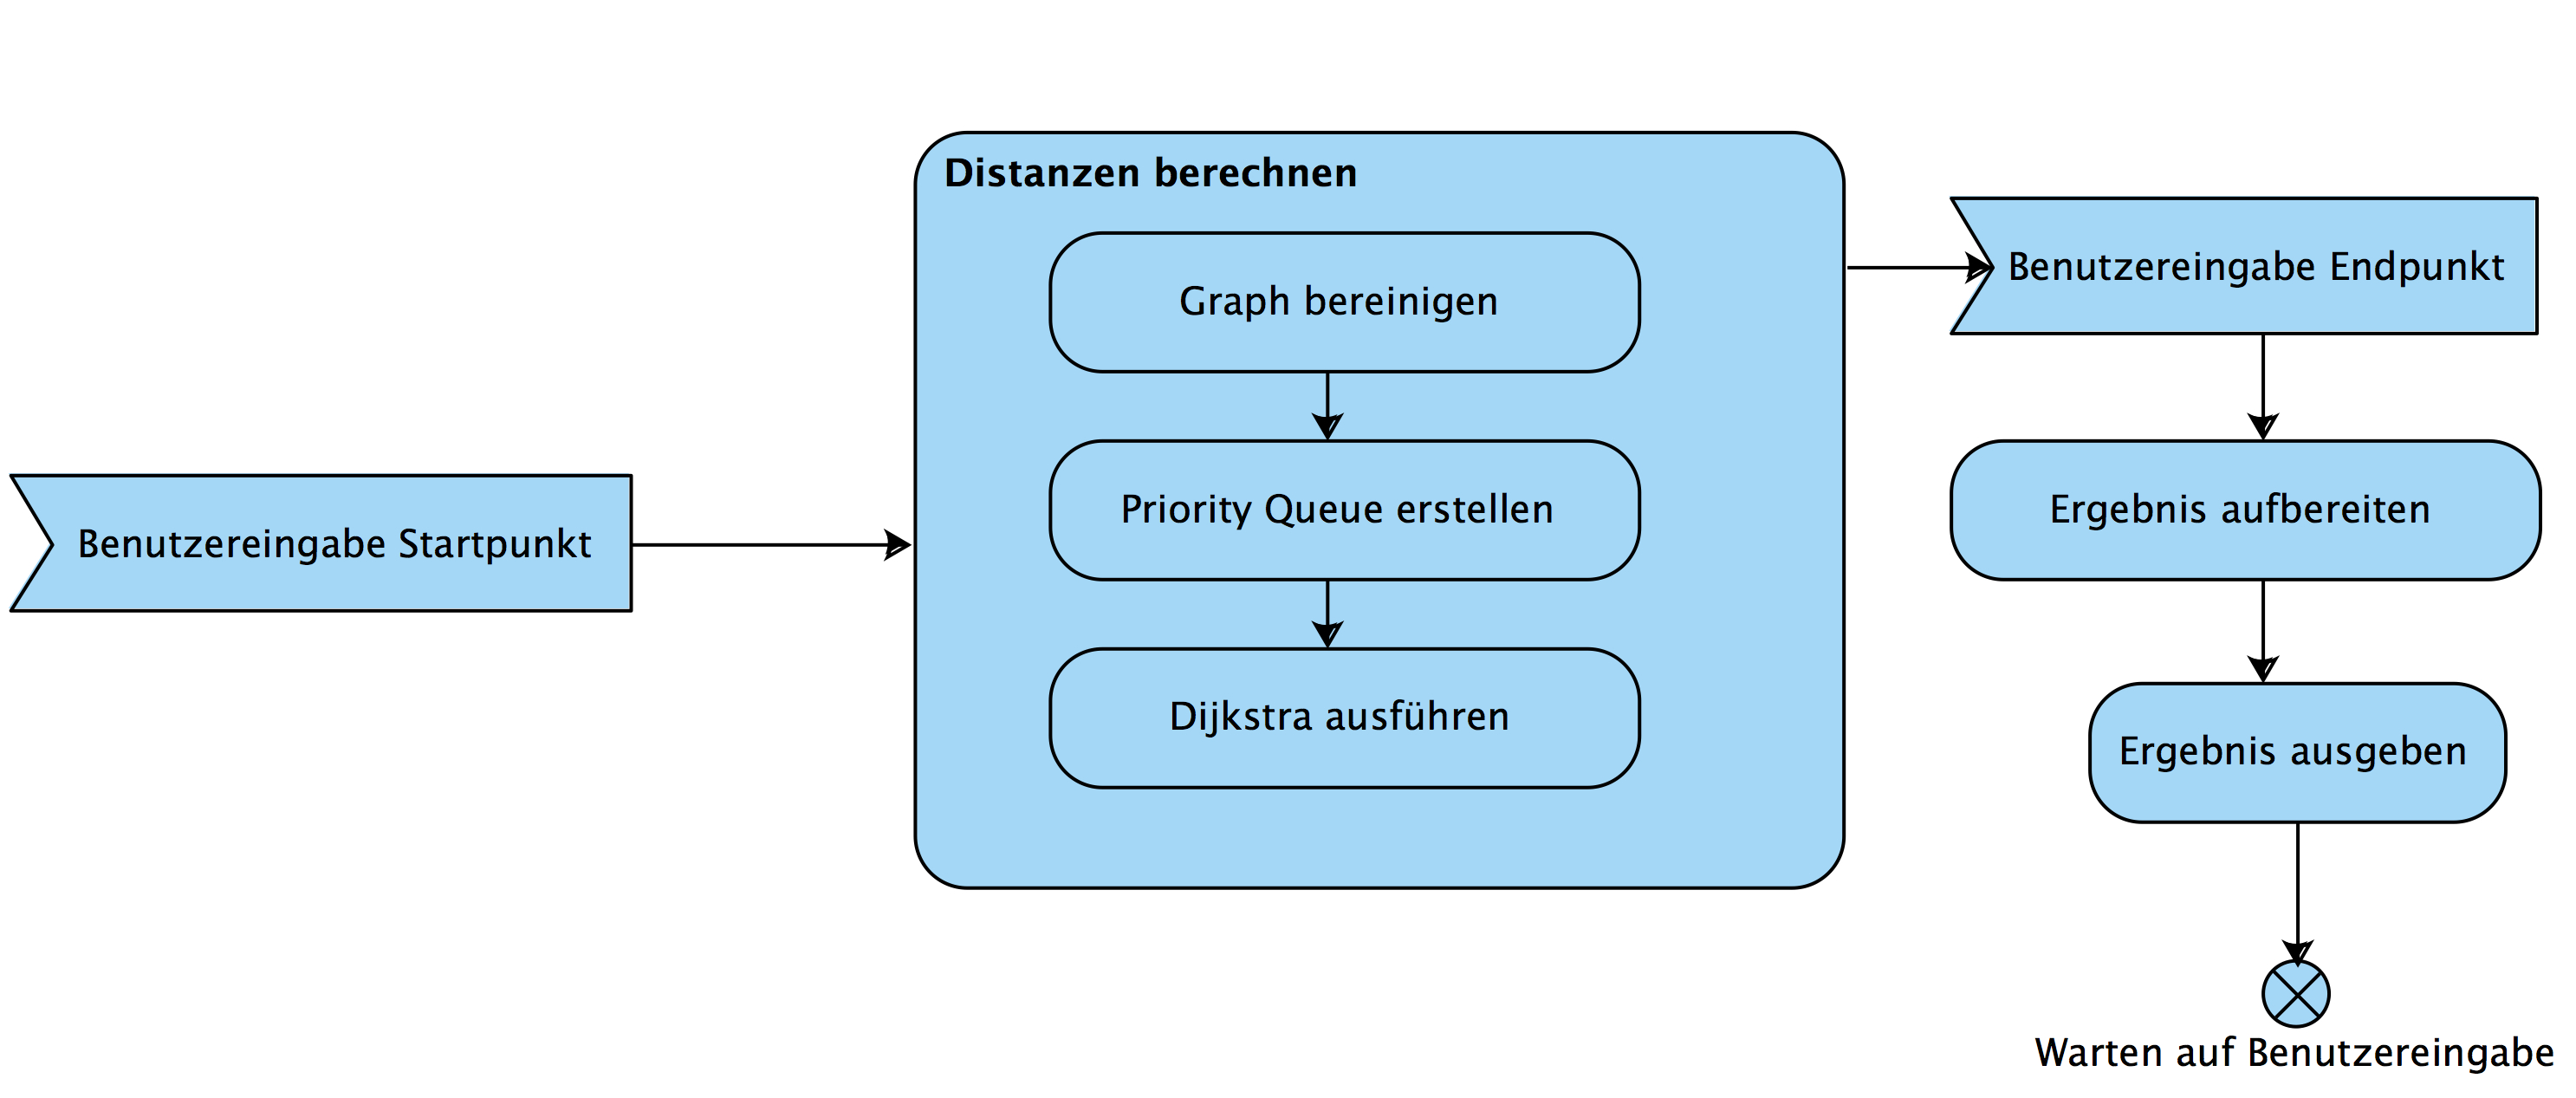
\includegraphics[width=1.0\textwidth]{Grafiken/aktivitaetsDiagrammDijkstra.jpg}
  \caption{Aktivitätsdiagramm der Routenberechnung}
  \label{fig:uebersichtRoutenberechnung}
\end{figure}

\subsubsection{Benutzereingabe Startpunkt}
Die Benutzerinteraktion ist in diesem Dokument nicht beschrieben. Verantwortlich für diese Interaktion ist die Klasse \textit{UserInterface}. Sie ist bewusst einfach gehalten und kann deswegen auch einfach geändert werden.

Um die Distanzen zu berechnen reicht der Startpunkt.

\subsubsection{Distanzen berechnen \label{distanzenBerechnen}}

\todo{Evebtuell hierfür eine Grafik basteln}

\paragraph{Graph bereinigen}
Vor Beginn der Distanzberechnung wird der Graph bereinigt. Bereinigen bedeutet, dass alle Knoten des Graphen bereinigt werden. Was beim Bereinigen geschehen muss:
\begin{itemize}
	\item Vorgänger: Der Knoten darf keinen Vorgänger besitzen. Hat ein Knoten einen Vorgänger, kann es bei der späteren Routenberechnung zu Fehlern kommen. Dem Attribut vorgänger des Knotens wird ein Nullpointer zugewiesen.
	\item Distanz: Die Distanz des Knotens wird mit der Konstante IN\_FINITY belegt. Diese Konstante ist auch intern von der Priority Queue benötigt.
	\item Besucht: Das Flag besucht des Knotens muss false gesetzt werden.
\end{itemize}

Dieser Schritt ist in der Dokumentation als ein eigener Schritt beschrieben. In der Release Version der Software wird dieser Schritt im Konstruktor der Klasse \textit{PriorityQueue} angestoßen.

\paragraph{Priority Queue erstellen \label{priorityQueueErstellen}}
Die Priority Queue ist das Herzstück unserer Implementierung des Dijkstra Algorithmus. Prinzipiell funktioniert sie, wie die formelle Beschreibung einer Priority Queue und basiert auf einer Map. Diese Implementierung bietet aber Methoden, die auf die Routenberechnung angepasst sind. 

Die Metrik der Queue ist die Distanz der Knoten, die noch nicht besucht wurden. Sind noch nicht besuchte Knoten in der Queue enthalten, wird beim Aufruf der \textit{getFirst()} Methode der Knoten zurück gegeben, der die kürzeste Distanz hat. Sind keine nicht besuchten Knoten mehr enthalten, wird ein Nullpointer zurück gegeben.

Beim Einfügen eines neuen Knotens prüft die Queue, ob dieser Knoten bereits in der Queue enthalten ist. Ist das nicht der Fall wird der Knoten eingetragen und relaxiert. Ist dieser Knoten bereits in der Queue enthalten, wird er nicht noch einmal hinzugefügt, sondern direkt relaxiert. Relaxieren bedeutet, dass geprüft wird, ob sich bei dem neuen Vorgänger eine Verbesserung der Distanz ergeben würde. Ist das der Fall, oder ist die alte Distanz IN\_FINITY, wird der neue Vorgänger des Knotens und die neue Distanz gesetzt. Das Flag besucht wird false gesetzt. Damit ist es möglich, dass der Knoten ein weiteres Mal von der Methode \textit{getFirst()} zurück gegeben werden kann und dass dessen Nachfolger mit der neuen Distanz relaxiert werden können.


\paragraph{Dijkstra ausführen}
Der Dijkstra Algorithmus basiert in unserer Implementierung auf der Priority Queue \ref{priorityQueueErstellen}. Die Methode die den Dijkstra Algorithmus implementiert durchläuft lediglich eine Schleife und trägt die Nachfolger des ersten Knoten aus der Priority Queue in diese ein. Diese Schleife wird terminiert, wenn die Queue einen Nullpointer zurück gibt. Nachdem diese Schleife durchlaufen ist, sind die Wege vom Startknoten zu sämtlichen Knoten berechnet.

%\todo{Ist der Graph eigentlich zusammenhängend? Ich glaube nicht, aber müssen wir das dokumentieren?}

\subsubsection{Benutzereingabe Endpunkt}
Um die Route bei gleichen Startpunkten und verschiedenen Zielpunkten nicht jedes Mal neu berechnen zu müssen, wurde die Aktivität \ref{priorityQueueErstellen} nur anhand des Startpunkts ausgeführt. Die Route wird berechnet, nachdem der Benutzer den Zielpunkt eingegeben hat.

\subsubsection{Ergebnis aufbereiten}
Die Aktion Ergebnis aufbereiten beinhaltet, dass vom Zielpunkt so lange durch die Vorgänger iteriert wird, bis der Startknoten erreicht ist. Diese Liste wird umgedreht und ans UserInterface zurückgegeben. Eine Berechnung findet an dieser Stelle nicht mehr statt.

\subsubsection{Ergebnis ausgeben}
Das Ergebnis wird dem Benutzer angezeigt.

\subsubsection{Warten auf Benutzereingabe}
Das Programm wartet eine Benutzereingabe. Möglich sind eine Neuberechnung der Strecken, die Ausgabe einer Route mit einem anderen Zielpunkt oder die Beendung des Programms.

\section{Pakete}
Das gesamte Programm besteht aus fünf Pakten. Die Klassen, die nicht primär am Programm beteiligt sind, werden an dieser Stelle nicht weiter erläutert. Die Dokumentation dieser Klassen befindet sich direkt im Quelltest, bzw. kann mit Doxygen ausgegeben werden.

In dieser Dokumentation sind \textit{deprecated} Methoden und Klassen nicht aufgeführt. Sie werden im Programm nicht (mehr) genutzt, sind aber weiterhin als Quellcode vorhanden und in der Doxygen Dokumentation entsprechend  dokumentiert.

\subsection{package:exceptions}
Dieses Pakt beinhaltet diverse Exceptions. 

\subsection{package:geopunkte}
In diesem Package sind alle Klassen enthalten, die unmittelbar mit den Lokationen bzw. deren Verwaltung zu tun haben.
\subsubsection{AttributDefines.h}
In dieser Headerdatei sind die Spalten definiert, in denen aus dem Originaldokument die entsprechenden Informationen ausgelesen werden können. Die Namen der Defines entsprechen denen, die in der Originaldokumentation des Bundes verwendet wurden. Im Kapitel \ref{attributBeschreibungen} ist beschrieben, wie die Originalnamen den im Programm verwendeten zugeordnet werden können. 

\subsubsection{Gebietslokation \label{class:Gebietslokation}}
Siehe \ref{AreaLocation}.

\subsubsection{Linearlokation \label{class:Linearlokation}}
Siehe \ref{linearLokation}.

\subsubsection{Punktlokation \label{class:Punktlokation}}
Siehe \ref{Punklokation}

\subsubsection{Lokationsverwaltung}
Diese Klasse beinhaltet eine Speicherstruktur und Methoden zu Verwalten der Lokationen. In der Speicherstruktur werden Pointer auf alle erstellten Lokationen gespeichert. Die Lokationen werden dynamisch allokiert, und im Destruktor dieser Klasse wieder destruiert. Ein Objekt dieser Klasse darf erst bei der Programmbeendung destruiert werden, da sämtliche Informationen über Lokationen hier verwaltet werden. Weiterhin enthält diese Klasse Methoden, die zum Erstellen (\ref{objekteErstellen}) der Lokationen benötigt werden.

\subsection{package:graph}
Im Package graph sind die Klassen enthalten, die unmittelbar an der Routenberechnung beteiligt sind.

\subsubsection{Dijkstra}
Diese Klasse beinhaltet Methoden zur Routenberechnung und um das Ergebnis der Routenberechnung aufzubereiten. 

\subsubsection{Graph}
Diese Klasse stellt den Graph dar und beinhaltet Methoden um ihn aufzubauen, sowie eine Datenstruktur um die Pointer auf die Knoten zu speichern. Der Aufbau des Graphen läuft in den Schritten \glqq Knoten erstellen \grqq und \glqq Knoten verlinken \grqq ab. Diese Unterteilung ist nötig, da die die Abhängigkeiten der Knoten untereinander durch Pointer dargestellt werden. Die Verlinkung der Abhängigkeiten kann nur erfolgen, wenn alle Knoten erstellt und deren Pointer bekannt sind.



\subsubsection{Knoten \label{class:Knoten}}
Die Klasse \textit{Knoten} stellt einen Knoten aus der Graphentheorie dar. In unserer Implementierung baut ein Knoten auf einer Punktlokation auf. Die Verbindungen zu den Punktlokationen werden durch einen Pointer auf die zugrundeliegende Punktlokation dargestellt. Diese Verbindung ermöglicht es, ohne zusätzlichen Speicheraufwand detaillierte Informationen zu dem Knoten zu bekommen. Zusätzlich zu den Grundinformationen hat ein Knoten Pointer auf seinen Vorgänger und seine Nachfolger. Der Vorgänger wird besonders wichtig, wenn aus den berechneten Distanzen eine Route gesucht werden soll. Die Nachfolger werden zur Berechnung der Distanzen benötigt. Weiterhin speichert ein Knoten seine Distanz zum Startknoten und ob er bereits besucht wurde. In \ref{priorityQueueErstellen} wurde beschrieben, wie diese Informationen verarbeitet werden.


\subsubsection{Priority Queue}
Diese Klasse bildet eine Priority Queue ab. Ihre Funktionsweise ist in \ref{priorityQueueErstellen} beschrieben. 

\subsection{package:hilfsklassen}
Dieses Paket beinhaltet eine Ansammlung von Klassen, die nicht direkt mit der Routenberechnung zu tun haben.
\subsubsection{Aktualitaet \label{class:Aktualitaet}}
Diese Klasse basiert auf dem \glqq tm *zeit\grqq~struct. Sie wird benötigt um das Attribut \ref{dt:aktualitaet} zu speichern und zu verwalten. Zusätzlich zu dem Struct bietet sie Methoden um die Zeit aus dem Datensatz auszulesen und zu validieren.

\subsubsection{Geokoordinate}
Diese Klasse wird für das Attribut \ref{st:geoKoordinate} benötigt. Sie enthält Methoden um aus einem String ein WGS84 Datum auszulesen, sowie mit GPS Daten zu rechnen. In ihr sind sowohl die X-Koordinate, als auch die Y-Koordinate des GPS Datums gespeichert.

\subsubsection{SicherLesen}
Dieses Header File bietet Funktionen um die grundsätzlichen Datentypen sicher über die Konsole einzulesen. Sicher bedeutet, dass der Eingabestrom überprüft und bei einem Fehler zurückgesetzt wird.


\subsubsection{UserInterface \label{UserInterface}}
Diese Klasse bietet dem User eine Schnittstelle zum Programm. Die Funktionen sind in \ref{Bedienungsanleitung} beschrieben.

\subsection{package:reader}
\subsubsection{FileOpener \label{class:FileOpener}}
Diese Klasse öffnet den Dateistream und zerlegt die .csv Datei in einen Vector. Das Verfahren ist in \ref{dateiOeffnen} beschrieben.

\subsection{Root Ordner}
Der Root Ordner des Programms enthält die Ordner mit den beschriebenen packages.

\subsubsection{Hello \label{hello}}
Diese Klasse ist die Main Klasse des Programms. In dieser Klasse wird die Dateiverarbeitung inklusive dem Konstruieren des Graphen initiiert. Der Dateipfad und -Name kann hier geändert werden. Zusätzlich wird hier das Benutzerinterface gestartet.


\section{Probleme bei der Routenberechnung \label{Probleme}}
\todo{Beispielsweise dass wir keine Ausfahrten im Datenbestand haben und dass die verlinkten Straßen auch weit auseinander liegen können }

\section{Anhang}
\subsection{Versionsdokumentation}
\subsubsection{Version 1.0.0}
Diese Version beinhaltet ein lauffähiges Programm. Fehler sind keine bekannt. Veröffentlicht am 07.06.2014
\subsubsection{Version 1.1.0}
Aus der Klasse \textit{LokationsVerwaltung} wurden die Datenstrukturen \textit{vector\textless Gebietslokation* \textgreater "-gebieteVector} und \textit{multimap \textless string, Gebietslokation* \textgreater namenMap} entfernt. Die Änderung ist in der Dokumentation berücksichtigt. Weiterhin sind Teile der Doxygen Dokumentation erweitert oder verbessert worden.

\subsubsection{Version 1.1.1}
Je nach Konstruktor der Prioirty Queue konnte die berechnete Distanz um -1 Kilometer abweichen. Dieser Fehler ist behoben.

\subsubsection{Version 1.2.0}
Die Makefiles wurden von Eclipse managed makefiles zu handgeschriebenen makefiles geändert. In sämtlichen Klassen wurde die Methode \textit{stoi} zu durch die Methode \textit{atoi} ersetzt.

\subsection{Attributliste \label{bundAttributListe}}
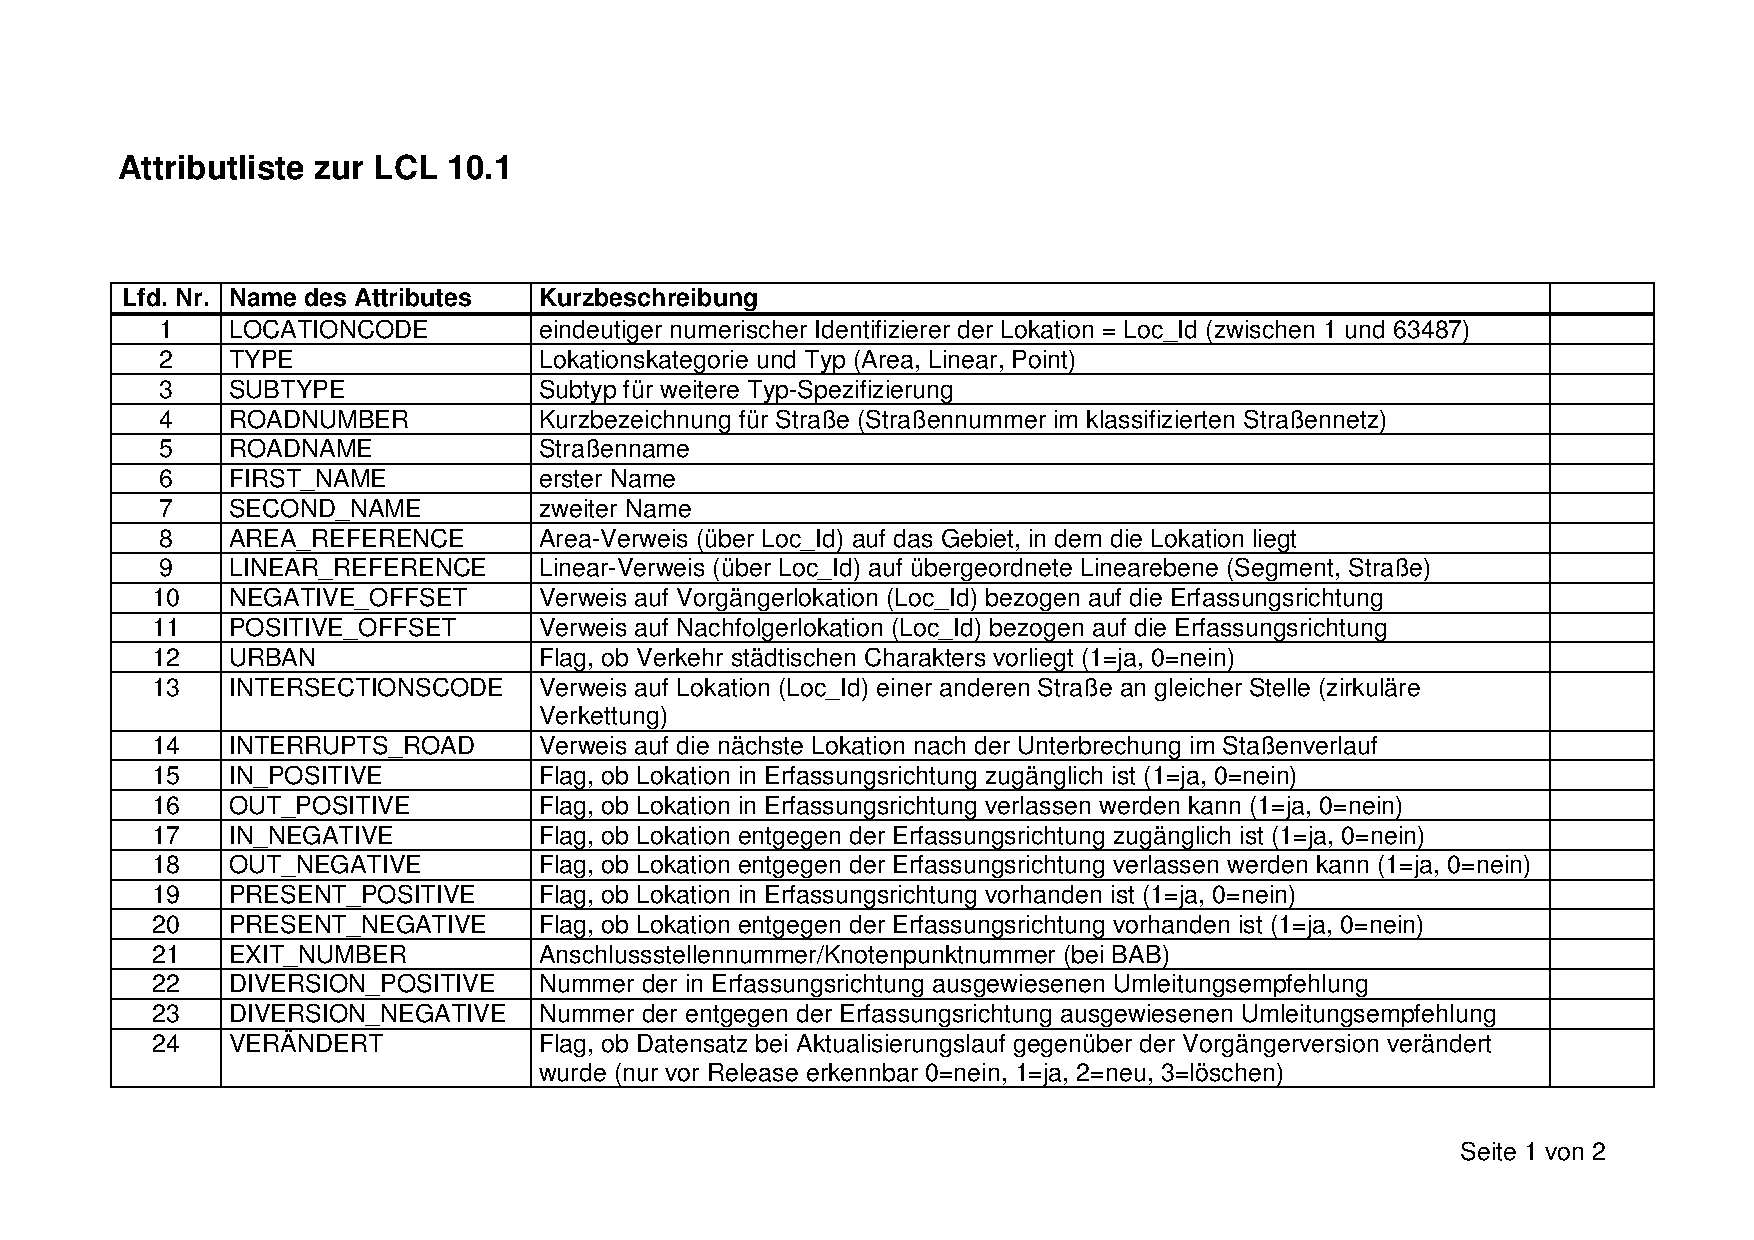
\includepdf[pages={1-2}]{Grafiken/RelatedDocuments/Attributliste_zur_LCL12.pdf}

\subsection{Typen und Untertypen der Lokationen \label{bundFeinDoku}}

\includepdf[pages={1-14}]{Grafiken/RelatedDocuments/Typenliste_V08_2010-03-03.pdf}

\subsection{Broschüre eines privaten Anbieters für Straßenverwaltungssoftware \label{bundGDD}}

\includepdf[pages=1-1]{Grafiken/RelatedDocuments/GDD-Strasse_PI.PDF}


\end{document}